



\section{Experimental Setup and Procedure}
\label{sec:Procedure}
In the following, the setup and the procedure of the experiment are described.
\subsection{Setup}
\label{sec:Setup}
The setup of this experiment is shown in \autoref{fig:set}. 
The whole apparatus is placed inside a vacuum chamber, 
since the $\alpha$ particles have a range of only about 1.5 cm in air \cite{Durchfuhrung}. The air is removed with a rotary vane pump.
\begin{figure}[htbp]
    \centering
    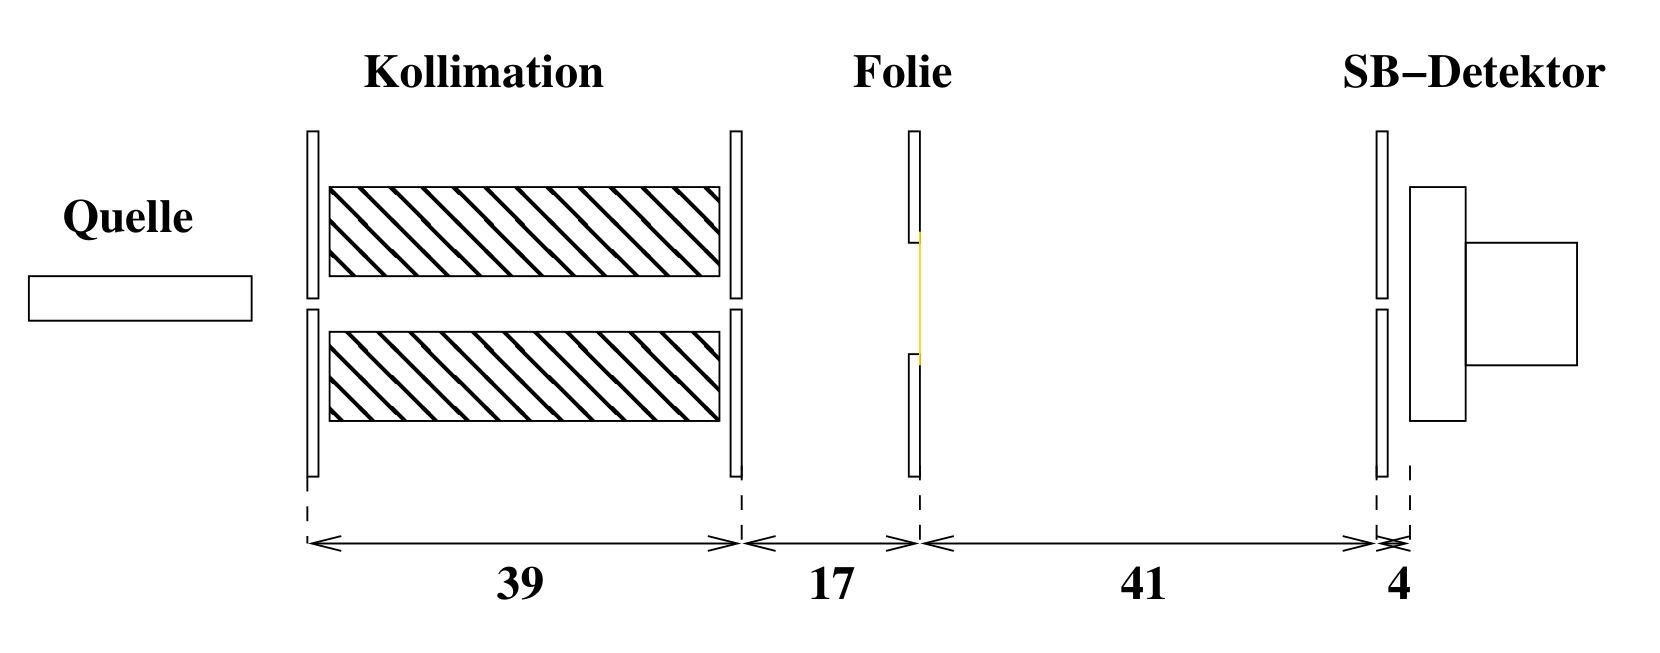
\includegraphics[width=0.75\textwidth]{v16/content/pics/setup.png}
    \caption{Scheme of the experimental setup, distances in mm. From left to right: source (Quelle), 
    collimator (Kollimation), foil (Folie) and surface barrier detector (SB-Detektor) with aperture. 
    Figure taken from \cite{Durchfuhrung}.}
    \label{fig:set}
\end{figure}
In this it is shown that the emitter is at the left, which is here the \ce{^{241}Am}, which produces the $\alpha$-particles. 
After the source, a collimator is placed, which puts the $\alpha$-particles on a straight path in the direction of the foil, 
by two $\SI{2}{mm}$ slits at the beginning and end of it, so only particles which are heading to the foil can go through. 
The collimiator is $\SI{39}{mm}$ long. 
After a distance of $\SI{17}{mm}$ the holder for the foil is placed. 
The source, the collimator, and the foil are mounted on a common holder, which can be rotated about an axis through the foil position. The detector stays fixed. The scattering angle $\theta$ is therefore the angle between the beam axis and the line from the foil to the detector, and it is set by rotating this holder.
Gold is especially good for this experiment because on the one hand it has a big nucleus and so a big cross-section and is 
on the other hand it is technically easy to produce in a thin layer. 
41 mm behind the foil, an aperture of $\SI{2}{mm}\times\SI{10}{mm}$ is placed, which defines the solid angle covered by the detector. The surface barrier detector is located 4 mm behind it \cite{Durchfuhrung}
This detector has a active area of $\SI{1}{cm^2}$ and a reverse bias voltage of $\SI{12}{V}$ is applied.
The signal of the surface barrier detector is proportional to the energy of the $\alpha$-particle, this signal is led into a preamplifier. 
The output of the preamplifier is fed into the main amplifier, which amplifies and shapes the pulses.
A discriminator passes only pulses above an adjustable threshold to the counter, so that only $\alpha$-particles are counted and noise and $\gamma$-rays are suppressed.

\subsection{Procedure}

To begin, the air will be pumped out of the probe chamber with the vane pump. 
After that, the real 0 angle will be measured by measuring without the foil and then measuring with different angles to get the angle where the most activation is measured. 
After determining this, that angle will be set as new 0. 
At this point the osziloskop will be connected one time after the preamplifier and after the amplifier so that the signal is readable. 
The signal after the preamplifier was not readable, and so this step was skipped. 
Then the discriminator was set up in a way that at room pressure, so that no $\alpha$-particles get to the detector, no counts are measured, 
because everything that did come through then, were $\gamma$-rays.
After this setup, the real measurements could start by measuring with the foil in the beam and setting the angle to different states. 
It was measured at big angles, so $30 \ge \theta \ge 5$, this has been done because at these angles the $\sin^4(\theta/2)$ dependencies are seen. 
The measurements are taken till approximately 1200 counts are measured so that the quality of it is comparable. 
The only exception is the measurement of an angle of $30°$ because this was measured over the night to get enough data. 
To get the rate, the counts were divided by the measuring time, which was always taken. 
\\
For the second real measurement, the air was still removed from the chamber, and a foil is inserted into the holder. 
Then the angle is set to the measured 0 so that the rate is the highest. 
Following this setup, the pressure in the chamber is slowly increased in steps, and in every step the height of the signal after the second amplifier is measured through an 
osziloskop. 
This process is repeated till the pressure in the chamber is at the outside pressure. 
After that, this measurement is repeated only without the foil. 

\clearpage